\section{Méthode de \textsc{Horn} et \textsc{Schunk}}

On fait l'hypothèse que le flot $h$ est régulier (au moins de classe $\mathscr{C}^2$ sur $\Omega = \interff{0}{1}^2$). On adopte une approche variationnelle du problème, et on se propose de déterminer le flot $h = (u,v)$ qui minimise l'énergie suivante sur $\Omega$:
\[ J(u,v) = \int_{\Omega} (I_xu + I_yv + I_t)^2 + \alpha^2\left( \abs{\nabla u}^2 + \abs{\nabla v}^2 \right) \]
où $\alpha$ est une constante réelle, et $I_\mu$ est la dérivée de $I$ par rapport à $\mu \in \lbrace x, y, t \rbrace$.\\
Si $\alpha = 0$, l'énergie est nulle quel que soit le flot $h$, donc la formulation variationnelle ne nous apprend rien...

\begin{enumerate}[questions]
\item On suppose que le minimum $(u,v)$ existe (dans un espace plus grand que $\mathscr{C}^2(\Omega)$). \\
On cherche un minimum dans $K = \mathscr{C}^2(\interff{0}{1}^2, \reels)$ (ou un ensemble de fonctions, ou de distributions, définies sur $\interff{0}{1}^2$), qui est un ensemble convexe. Montrons que la fonctionnelle $J$ est strictement convexe sur $K$.\\
Soient $(u_1, v_1) \neq (u_2, v_2) \in K$ et $\lambda \in \interoo{0}{1}$.
\begin{multline*}
J((1-\lambda)(u_1, v_1) + \lambda(u_2, v_2)) = \\
\int_{\Omega} \left[ \left( \left(1-\lambda\right) \left( I_x u_1 + I_y v_1 + I_t \right) + \lambda \left( I_x u_2 + I_y v_2 + I_t \right) \right)^2 \right. \\
\left. + \alpha^2 \left( \abs{(1-\lambda)\nabla u_1 + \lambda \nabla u_2}^2 + \abs{(1-\lambda)\nabla v_1 + \lambda \nabla v_2}^2 \right) \right]
\end{multline*}
Or, la fonction $x \mapsto x^2$ est strictement convexe sur $\reels$, donc :
\begin{multline*}
\left( \left(1-\lambda\right) \left( I_x u_1 + I_y v_1 + I_t \right) + \lambda \left( I_x u_2 + I_y v_2 + I_t \right) \right)^2 \\
< (1-\lambda)\left( I_x u_1 + I_y v_1 + I_t \right)^2 + \lambda \left( I_x u_2 + I_y v_2 + I_t \right)^2
\end{multline*}
De même, la fonction $x \mapsto \abs{x}^2$ est strictement convexe sur $\reels^d$ (comme somme de $d$ fonctions strictement convexes), donc :
\[ \abs{(1-\lambda)\nabla u_1 + \lambda \nabla u_2}^2 < (1-\lambda)\abs{\nabla u_1}^2 + \lambda\abs{\nabla u_2}^2 \]
et de même avec $v_1$ et $v_2$.\\
\itshape N.B. --- Ces inégalités sont écrites en tout point $(x,y) \in \Omega$, omis pour alléger l'écriture.\\ \upshape
Finalement, on a:
\[ \forall \lambda \in \interoo{0}{1}, \quad J((1-\lambda)(u_1, v_1) + \lambda(u_2, v_2)) < (1-\lambda)J(u_1, v_1) + \lambda J(u_2, v_2) \]
ce qui traduit que $J$ est strictement convexe sur $K$.\\
D'après la proposition 4.1.6 p. 106 du polycopié de cours, \emph{le minimum est global et unique}.


\item On note $\bar{h} = (\bar{u}, \bar{v})$ le flot minimisant. Pour tout $u$ on a donc:
\begin{align*}
J(\bar{u}+u, \bar{v}) &= \int_{\Omega} (I_x(\bar{u}+u) + I_y\bar{v} + I_t)^2 + \alpha^2\left( \abs{\nabla (\bar{u}+u)}^2 + \abs{\nabla \bar{v}}^2 \right) \\
&= J(\bar{u}, \bar{v}) + \int_\Omega \left[2 I_x u(I_x\bar{u} + I_y\bar{v} + I_t) + 2\alpha^2 \nabla\bar{u} \cdot \nabla u\right] + \alpha^2 \int_\Omega \abs{\nabla u}^2
\end{align*}
Le terme central est la différentielle partielle de $J$ par rapport à sa première coordonnée, en $\bar{h}$, évaluée en $(u, 0)$, donc comme $\bar{h}$ minimise $J$, on peut affirmer que:
\[ \forall u, \qquad \int_\Omega \left[I_x u(I_x\bar{u} + I_y\bar{v} + I_t) + \alpha^2 \nabla\bar{u} \cdot \nabla u\right] = 0 \]
On peut en particulier choisir $u$ dans $\mathscr{C}^\infty(\Omega)$. Par application de la formule de \textsc{Green-Riemann}, on obtient:
\[ \forall u \in \mathscr{C}^\infty(\Omega), \qquad \int_\Omega u\left[I_x(I_x\bar{u} + I_y\bar{v} + I_t) - \alpha^2 \Delta\bar{u} \right] = 0 \]
Le lemme 3.1.7 du cours permet d'affirmer alors que:
\[ I_x(I_x\bar{u} + I_y\bar{v} + I_t) - \alpha^2 \Delta\bar{u} = 0 \quad \text{sur } \Omega \]

On tient le même raisonnement en évaluant la différentielle de $J$ au point $\bar{h}$ calculée au point $(0, v)$. On obtient donc le système d'équations suivant:
\begin{equation}
\begin{cases*}
I_x^2 u + I_xI_y v = \alpha^2 \Delta u - I_xI_t \\
I_xI_y u + I_y^2 v = \alpha^2 \Delta v - I_yI_t 
\end{cases*} \label{eq:syst}
\end{equation}

\item On \og{}prolonge\fg{} les matrices $I$ à $\relatifs^2$ par le procédé suivant:
	\[ \begin{array}{cc|ccc|cc}
	\ddots & \vdots & \vdots & & \vdots & \vdots & \iddots \\
	\dots & I_{11} & I_{11} & \dots & I_{1N} & I_{1N} & \dots \\ \hline
	\dots & I_{11} & I_{11} & \dots & I_{1N} & I_{1N} & \dots \\
	 & \vdots & \vdots & \ddots & \vdots & \vdots &  \\
	\dots & I_{N1} & I_{N1} & \dots & I_{NN} & I_{NN} & \dots \\ \hline
	\dots & I_{N1} & I_{N1} & \dots & I_{NN} & I_{NN} & \dots \\
	\iddots & \vdots & \vdots & & \vdots & \vdots & \ddots
	\end{array} \]
Le code de la fonction se trouve dans le fichier \verb|functions.sci|, et la fonction correspondante s'appelle \verb|derivees|.

\item Pour calculer la moyennée de la matrice $U$, on la prolonge d'abord sur ses quatre \og{}côtés\fg{} comme ceci:
	\[ \begin{array}{|c|ccc|c|}
	\hline
	U_{11} & U_{11} & \dots & U_{1N} & U_{1N} \\ \hline
	U_{11} & U_{11} & \dots & U_{1N} & U_{1N} \\
	\vdots & \vdots & \ddots & \vdots & \vdots \\
	U_{N1} & U_{N1} & \dots & U_{NN} & U_{NN} \\ \hline
	U_{N1} & U_{N1} & \dots & U_{NN} & U_{NN} \\ \hline
	\end{array} \]
On applique alors la formule proposée dans l'énoncé à cette nouvelle matrice notée $\hat{U}$. Enfin, on extrait la sous-matrice (\og{}notation Scilab\fg{}):
\[ \bar{U} = \hat{U}_{2:N+1, 2:N+1} \]
L'implémentation est faite dans la fonction \verb|moyenneMat| du fichier \verb|functions.sci|.

\item Afin de résoudre numériquement le système d'équations~(\ref*{eq:syst}) \vpageref{eq:syst}, on approche le laplacien par une fonction plus simple.

En effet, la formule de \textsc{Taylor-Young} nous donne:
\[ u(x+h, y+k) = u(x,y) + h \partial_xu + k \partial_yu + \dfrac{h^2}{2}\partial^2_{xx}u + hk \partial^2_{xy}u + \dfrac{k^2}{2}\partial^2_{yy}u + O(h^3 + k^3) \]

Par définition, on a:
\[ \bar{u}_{i,j} = \dfrac{1}{6}\left( u_{i-1,j} + u_{i+1,j} + u_{i,j+1} + u_{i,j-1} \right) + \dfrac{1}{12}\left( u_{i-1,j-1} + u_{i-1,j+1} + u_{i+1,j-1} + u_{i+1,j+1} \right) \]
On écrit dorénavant $u$ au point $(i,j)$:
\begin{multline*}
\bar{u} \simeq \dfrac{1}{6} \left( u - \partial_xu + \frac{1}{2}\partial^2_{xx}u + u + \partial_xu + \frac{1}{2}\partial^2_{xx}u + u + \partial_yu + \frac{1}{2}\partial^2_{yy}u + u - \partial_yu + \frac{1}{2}\partial^2_{yy}u \right) \\
+ \dfrac{1}{12} \left( u - \partial_xu - \partial_yu + \frac{1}{2}\partial^2_{xx}u + \partial^2_{xy}u + \frac{1}{2}\partial^2_{yy}u + \cdots \right. \\
\left. + \dots + u + \partial_xu + \partial_yu + \frac{1}{2}\partial^2_{xx}u + \partial^2_{xy}u + \frac{1}{2}\partial^2_{yy}u \right)
\end{multline*}
d'où, après simplification:
\[ \bar{u} \simeq u + \dfrac{1}{3}\Delta u \iff \Delta u \simeq 3(\bar{u} - u) \]

On peut alors réécrire le système (\ref{eq:syst}) \vpageref{eq:syst}:
\[ 
\begin{cases*}
I_x^2u + I_xI_yv = \alpha^2(\bar{u} - u) - I_xI_t \\
I_xI_yu + I_y^2v = \alpha^2(\bar{v} - v) - I_yI_t
\end{cases*}
\iff 
\begin{cases*}
(I_x^2 + \alpha^2)u + I_xI_yv = \alpha^2\bar{u} - I_xI_t \\
I_xI_yu + (I_y^2 + \alpha^2)v = \alpha^2\bar{v} - I_yI_t
\end{cases*}
\]

Ce dernier système se réécrit matriciellement:
\[
\begin{pmatrix}
I_x^2 + \alpha^2 & I_xI_y \\
I_xI_y & I_y^2 + \alpha^2
\end{pmatrix}
\begin{pmatrix}
u \\ v
\end{pmatrix} = 
\begin{pmatrix}
\alpha^2\bar{u} - I_xI_t \\
\alpha^2\bar{v} - I_yI_t
\end{pmatrix} \iff
A
\begin{pmatrix}
u \\ v
\end{pmatrix} = b
\]
Le déterminant de la matrice  $A$ est égal à $\alpha^2(\alpha^2 + I_x^2 + I_y^2) > 0$ donc $A$ est inversible. On a alors:
\[ \begin{pmatrix}
u \\ v
\end{pmatrix} = A^{-1}b = 
\begin{pmatrix}
\bar{u} - I_x \dfrac{I_x\bar{u} + I_y\bar{v} + I_t}{\alpha^2 + I_x^2 + I_y^2} \\
\bar{v} - I_y \dfrac{I_x\bar{u} + I_y\bar{v} + I_t}{\alpha^2 + I_x^2 + I_y^2}
\end{pmatrix}
\]

On peut considérer cette égalité comme une équation linéaire de la forme $I_2X = B$ avec $I_2$ la matrice identité d'ordre 2 et $B$ un vecteur de $\reels^2$. L'identité est à diagonale dominante, donc on peut appliquer le schéma de Jacobi:
\[ I_2X_{n+1} = 0_2X_n + B_n \]
où $0_2$ est la matrice nulle d'ordre 2, soit encore:
\[ \begin{cases*}
u^{n+1} = \bar{u}^n - I_x \dfrac{I_x\bar{u}^n + I_y\bar{v}^n + I_t}{\alpha^2 + I_x^2 + I_y^2} \\
v^{n+1} = \bar{v}^n - I_y \dfrac{I_x\bar{u}^n + I_y\bar{v}^n + I_t}{\alpha^2 + I_x^2 + I_y^2}
\end{cases*} \]

\item On implémente l'algorithme dans le fichier \verb|functions.sci|, avec la fonction \verb|flow| qui prend en entrée les matrices des images et affiche le flot calculé dans un graphique. On l'a testé avec les images ci-dessous.
\begin{figure*}[!h]
\centering
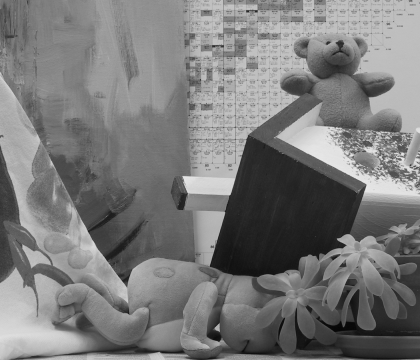
\includegraphics[width=.45\textwidth]{img/q7-orig-1}
\hfill
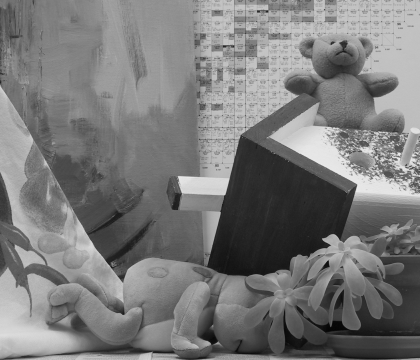
\includegraphics[width=.45\textwidth]{img/q7-orig-2}
\end{figure*}

On voit que les zones présentant de fortes discontinuités de luminosité sont bien traitées : le flot est bien défini en direction, et il est distribué de façon homogène. En revanche, dans les zones uniformes, le flot est erratique et ne permet de conclure quant au mouvement des points matériels représentés (cf.~figure~\vref{fig:q7-results}).
\begin{figure}[!h]
\centering
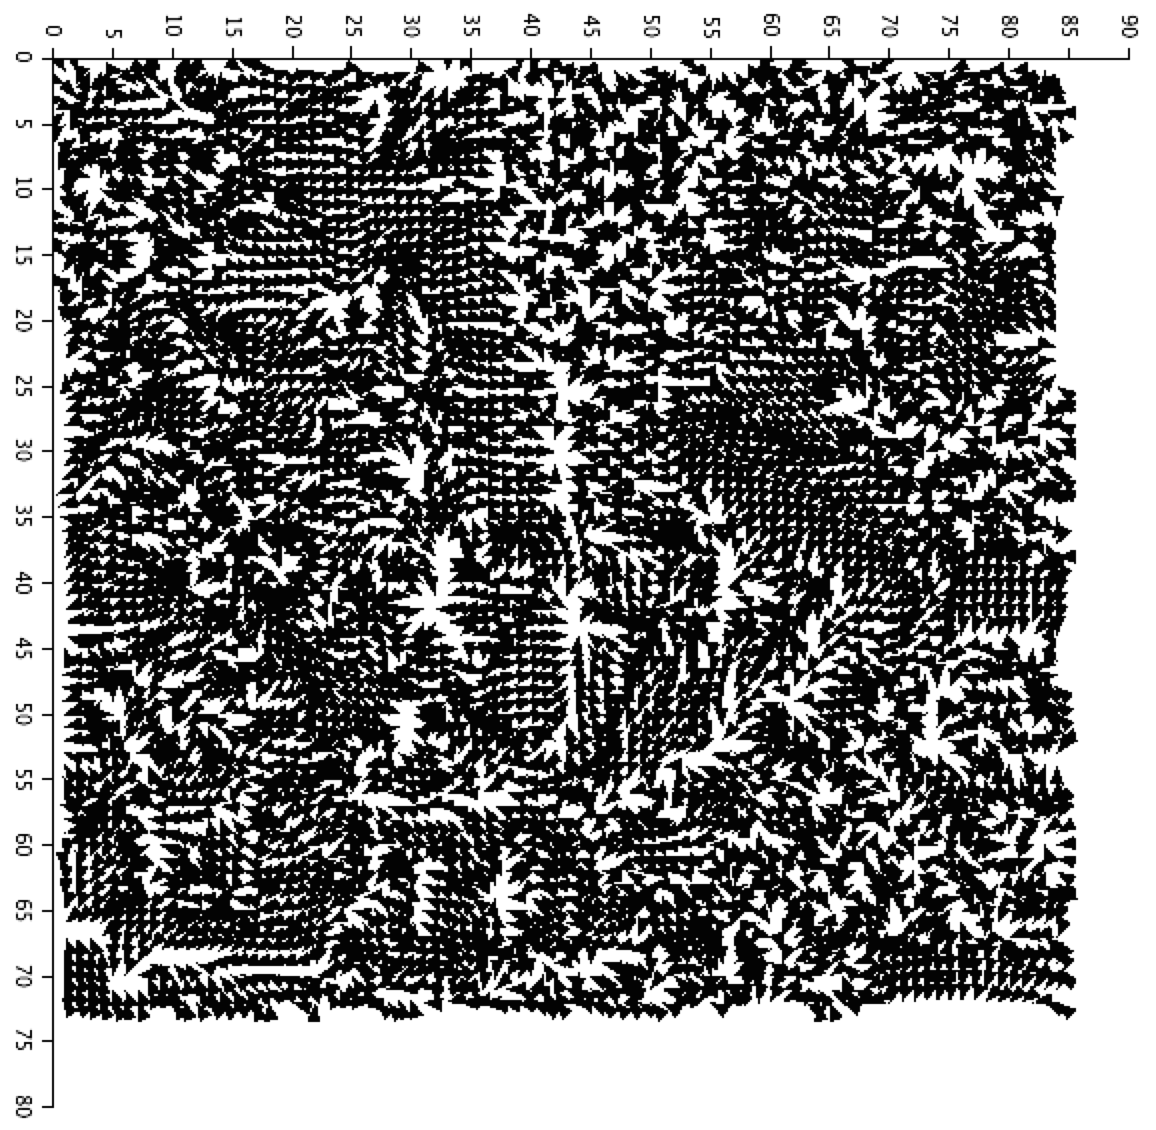
\includegraphics[width=.65\textwidth]{img/q7-results}
\caption{Résultat de la question 7.\label{fig:q7-results}}
\end{figure}
\end{enumerate}